\documentclass[12pt]{report}

\usepackage{graphicx}
\usepackage{textcomp}
\usepackage[margin=1.0in]{geometry}
\usepackage[symbol]{footmisc} % Used to have symbols for footnotes instead of numbers (so as to not get confused between references and footnotes)
\usepackage{gensymb} % Used for the degree symbol in math mode
\usepackage[subrefformat=parens,labelformat=parens]{subfig} % Used to combine figures into one
\usepackage{cleveref} % Makes references easier
\usepackage{bm} % Used for bold font in math mode
\usepackage[superscript,biblabel,sort]{cite} % The superscript option puts the references as superscript numbers, biblabel applies the superscript to the references page, and sort sorts the numbers from least to greatest, and if possible, puts a dash to shorten it (i.e. 1,2,3,4,5,6 will be shortened to 1-6)

\bibliographystyle{aip2}

% This is the Introduction and Background section of the paper
\begin{document}
\chapter{Introduction\label{intro}}
Uranium dioxide (UO\textsubscript{2}) is the primary choice for nuclear fuel in today's reactors.\cite{uraniumInfo}  In order to understand the properties of UO\textsubscript{2}, an analysis of the basic crystal structure of the material is required.  UO\textsubscript{2} is a ceramic, meaning that a series of crystal lattices join together in various ways (called twist, tilt, or mixed boundaries) to create the material.  This material has a fluorite crystal structure, where the uranium atoms form a face-centered cubic (fcc) lattice, and the oxygen atoms form a simple cubic lattice within the fcc frame (see \Cref{fig:uo2Lattice}).

For a nuclear reactor to work properly, many things need to be taken into consideration.  First, understanding the ideal operating conditions for the nuclear reactor is important so immediate actions can be taken when conditions are no longer ideal.  Radioactivity has an effect on all materials, not just living tissue.  Over time, radiation can create defects in the crystal structures of the metals used to create the reactor shell, and these defects can build up, causing deformation, weakening, or stiffening of the materials, which can lead to problems if not properly managed.\cite{callister2003}.  As the reactions continue, more neutrons are created, potentially causing additional fission events.  To prevent the reactor from having all the fuel fission at nearly the same time (releasing a large amount of energy), various methods control the number of chain reactions.  Emergency procedures also prevent catastrophes such as the ones that occurred at Three Mile Island, Chernobyl, and Fukushima.

Second, the quality of the fuel must meet a minimum standard for a sustainable reaction to occur.  Nuclear fuels come in one of two categories: fissile, where bombardment of the material with neutrons will divide the atomic nuclei into ``daughter" particles, releasing energy, and non-fissile, where bombardment of the material results in the neutrons becoming part of the nucleus, called absorption.  Nuclear reactors require fissile materials to work.  One of the most common fissile materials is an isotope of uranium called U-235.  A second isotope of uranium, U-238, is much more common (approximately 99\% of all uranium).  Sustainable chain-reactions have at least a minimum amount of U-235 present in the fuel, depending on the moderating medium.\cite{uraniumInfo}

Third, the various properties of the fuel need to be well understood to make running the reactor as safe and effective as possible.  Some of these properties include thermal conductivity (how well heat flows through the material), fission gas release (how some of the fission products move throughout the material as gases), and mechanical stability (i.e. how the material bends or cracks under pressure or heat).  Taking thermal conductivity as an example, knowledge of this material property allows the most effective use of coolant to keep the reactor within operating temperatures, maximizing both efficiency and safety.  Knowledge of other material properties allows for similar gains in efficiency, safety, or both.


This work adds to the safety and efficiency of using nuclear energy by providing the necessary information to accurately calculate the material properties of UO\textsubscript{2} in-reactor.  Specifically, this work improves the fitting parameters for grain boundary (GB) energy interpolation for UO\textsubscript{2} by using molecular dynamics (MD) results calculated by Zhang\cite{zhang2016} and Hansen\cite{hansen2016} with an anneal of 800 K.  Previous data did not anneal the crystal structure\cite{harbison2015}, which prevented the atoms from finding their ideal energetic minimum.  The 800 K anneal allows the atoms to relax to a value closer to their global minimum, as shown in \Cref{results}.  A database will store these simulated energies, and a MATLAB\textsuperscript{\textregistered} script will use the database to fit the function parameters.  Idaho National Laboratory (INL) will incorpoate the updated parameters into its mesoscale phase field modeling platform MARMOT for use in modeling nuclear fuels.  As these parameters are implemented in the modeling software, various tests of the UO\textsubscript{2} fuel can determine how the material properties change while in-reactor.

\begin{figure}[ht!]
\centering
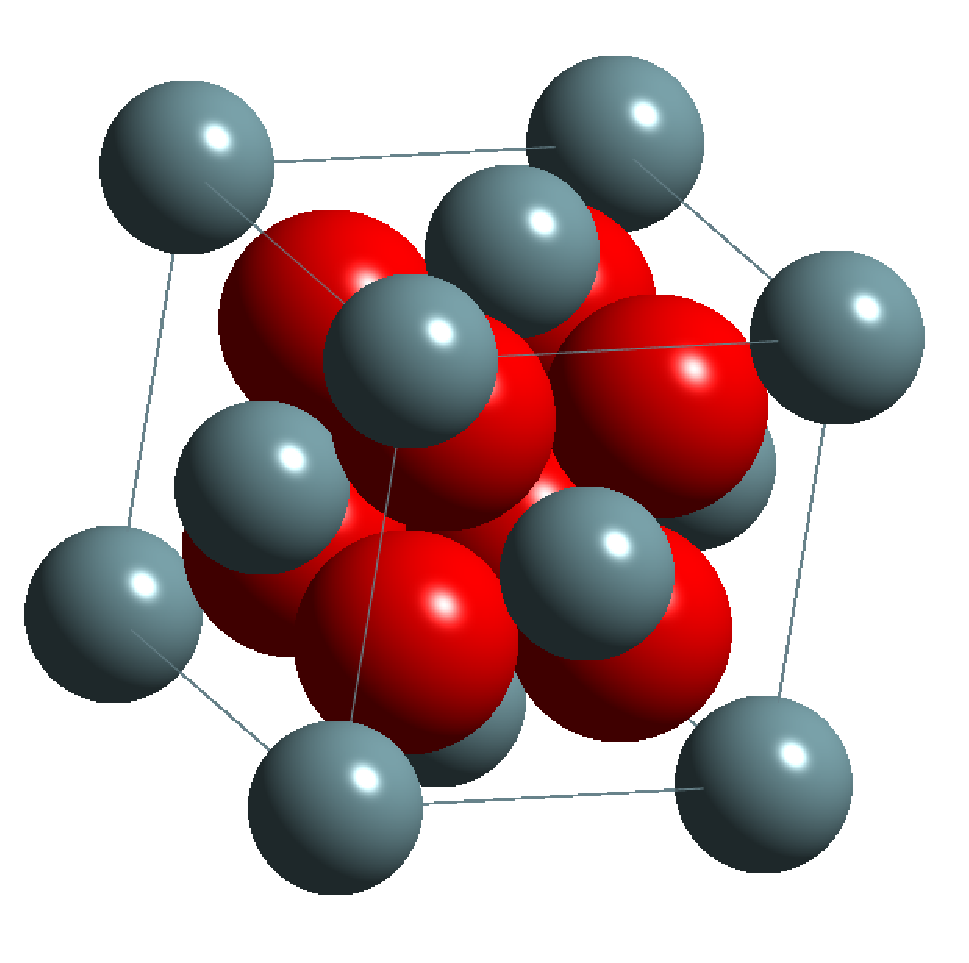
\includegraphics[scale=1.0]{Images/UO2}
\caption[Example of the fluorite crystal structure.]{\label{fig:uo2Lattice}An image representing the fluorite crystal structure.  For UO\textsubscript{2}, the smaller spheres indicate the uranium atoms, and the larger spheres indicate the oxygen atoms.  Image courtesy of the University of Cambridge under the Creative Commons license.}
\end{figure}

\section{Background\label{intro:background}}
Polycrystalline materials (ceramics, metals, and polymers) are composed of tiny crystals called \emph{grains}.  The orientation of each grain is generally independent of the orientation in the grains surrounding it. Therefore, there is a possibility (depending on how the crystal formed\cite{callister2003}) that crystal structures will not line up at the interfaces where these two grains meet.  This ``atomic mismatch"\cite{callister2003} leads to broken or stretched atomic bonds where atoms will not line up relative to a perfect crystal structure.  These defects are called grain boundaries (GBs), and an illustration of a GB is shown in \Cref{fig:gb}. The most popular way to parameterize a GB uses the five degree-of-freedom (DoF) model.\cite{patala2013, lejcek2010, homer2015, bulatov2014, harbison2015, rohrer2011}.  This model only uses the macroscopic DoFs (the observable DoFs corresponding to the misorientation and inclination), ignoring the three translational DoFs (the ability of the grain to move or slide anywhere in space) possessed by each grain.  Three of the five DoFs specify the misorientation (or misaligment) of the grains with respect to each other.  The other two DoFs specify the orientation of the grain boundary plane (called the inclination).  The misorientation DoFs consist of the rotation angle $\theta$ (one of three) and the rotation axis (another two angles, where the first angle is measured in the $xy$-plane perpendicular to the $z$ axis, and the second angle is measured from the positive $z$-axis), while the normal of the GB defines the inclination DoFs (two angles).\cite{lejcek2010}

Three specific types of GBs occur in polycrystalline materials: twist, tilt, and mixed GBs.\cite{lejcek2010, rohrer2011}  These GBs desribe the misorientation of two grains with respect to each other.  Twist boundaries have the axis of rotation between the two grains and the GB normal parallel to each other. Tilt boundaries can be either symmetric and asymmetric.  A tilt boundary occurs when the axis of rotation between the two grains is perpendicular to the GB normal.  Symmetric tilt boundaries describe a GB whose boundary plane is a mirror plane: one side of the boundary mirrors the other.  This makes the angles between the boundary plane and the orientation axes of the two grains equal. Asymmetric tilt boundaries have unequal angles.  \Cref{fig:misorientation} shows a representation of tilt boundaries (top) and twist boundaries (bottom).  A mixed GB is a combination of twist and tilt boundaries in some degree.

Understanding GBs is important because of the effects they have on material properties.\cite{patala2013, homer2015, bulatov2014}  The crystal structure has extra energy because of the atomic mismatch at the boundaries.  This extra energy, called GB energy, gives rise to GB motion.  Knowing and predicting how the GBs will move allows for more accurate calculations of a material's properties.  Thus, GB energy needs to be understood to accurately model the evolution of material properties.

Two methods of modeling GB energy are the isotropic and anisotropic models.  The most common method (and easier method) is the isotropic model.  This model ignores the impact of inclination on the GB energy, and assumes equal inclinations for a given misorientation, reducing the five-dimensional (5D) parameter space to a three-dimensional (3D) parameter space.  The reasons for assuming this model historically was based on the assumption that the inclination had little or no impact on the GB energy, or (later) that it was too difficult to create a full five DoF model.\cite{homer2015}  Alternatively, the anisotropic approach seeks to quantify the effect that misorientation \emph{and} inclination have on the GB energy.  Currently researchers acknowledge the need for a full five DoF model for the GB energy, but assert the difficulty inherent in developing such a model.\cite{rohrer2011, lejcek2010, homer2015}  Despite these difficulties, GB energy functions for certain materials, namely fcc metals copper, gold, aluminum, and nickel, have proven successful.\cite{bulatov2014}

\begin{figure}[ht!]
 \centering
 
 \subfloat[]{\label{fig:gb}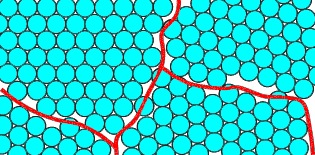
\includegraphics[scale=.9]{Images/grainBoundary}}\quad
 \subfloat[]{\label{fig:misorientation}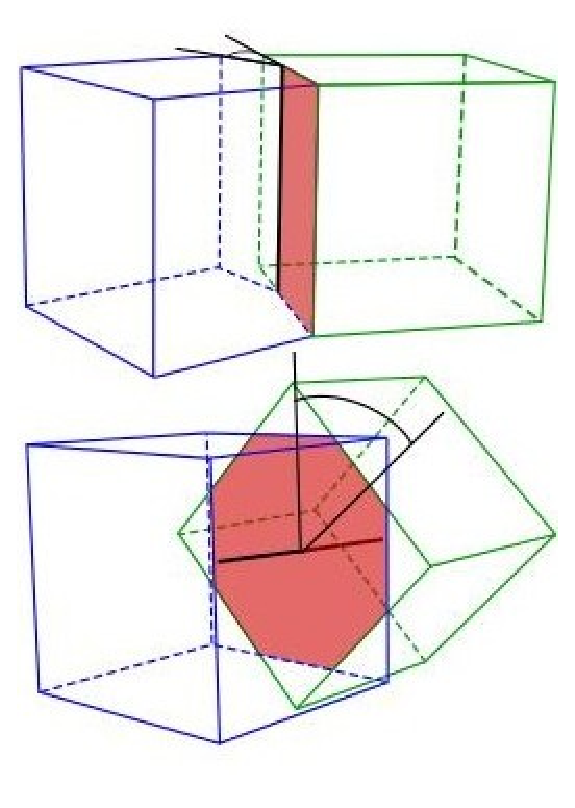
\includegraphics[scale=.6]{Images/twistTilt}}\quad
 \caption[Examples and types of grain boundaries.]{\label{gbs} A representation of GBs, where \protect\subref{fig:gb} shows an example of a grain boundary and \protect\subref{fig:misorientation} shows an example of GB types.  In \protect\subref{fig:gb} circles represent individual atoms of the grains, and the line represents the grain boundary.  Atomic mismatch between the differently oriented grains causes an excess of energy within the material, which has an effect on the material's properties.  Image courtesy of the University of Cambridge under the Creative Commons license. In \protect\subref{fig:misorientation} the axis of rotation for the tilt GB (top) is perpendicular to the GB normal, and for the twist GB (bottom) is parallel to the GB normal.  Image courtesy of Wikipedia under the Creative Commons license.}
\end{figure}

\section{Previous Work\label{intro:prevWork}}
Bulatov \emph{et al.}\cite{bulatov2014} developed a five DoF function which accurately interpolates GB energies for certain fcc metals.  They used energies for GBs along specific axes to interpolate the full 5D GB space.  \Cref{methods} explains their methods in more detail.  Harbison\cite{harbison2015} applied Bulatov \emph{et al.}'s methods to calculate similar parameters to describe the full five DoF GB space for UO\textsubscript{2}.  GB energies for various misorientations around a high-symmetry axis were gathered using MD simulations.  The fitting procedure created a set of 43 parameters defining the function needed to interpolate an arbitrary GB energy.
\bibliography{gbCharacter}
\end{document}